% Compile twice with pdflatex from the repo root.
\documentclass[aspectratio=169,11pt]{beamer}
\usetheme{Warsaw}\usecolortheme{default}
\usepackage[T1]{fontenc}
\usepackage{lmodern,amsmath,booktabs,tabularx,graphicx,tikz}
\usetikzlibrary{arrows.meta,positioning}
\definecolor{afgml}{RGB}{22,57,86}
\setbeamercolor{structure}{fg=afgml}
\setbeamertemplate{navigation symbols}{}
\setbeamertemplate{footline}[frame number]
\newif\ifguidance\guidancefalse
\newcommand{\help}[1]{\ifguidance\begin{block}{Preparation guidance}\small #1\end{block}\fi}
\newcommand{\fillin}[1]{[\textit{#1}]}
\title[AFGML Capstone]{Fairness Preservation under Computational Budgets in Probabilistic Decision Systems}
\subtitle{ICT 5143: AFGML Capstone | Problem 9}
\author{Shreeya Kamath (261090830022) \and Misha (261090830020)}
\date{7 November 2026}
\begin{document}
\begin{frame}\titlepage\end{frame}

\begin{frame}{Research question and decision context}
\begin{itemize}
\item Context and stakeholders: bank outreach scored by a Bayesian network under a compute limit; affected are customers, outreach teams, serving engineers and auditors.
\item $Y=1$: recorded term-deposit subscription; $D=1$: selected for \emph{hypothetical} pre-contact outreach (top 20\% of scores).
\item Question: at a fixed operation budget, does choosing the fallback by validation worst-group deviation from the exact decision give a smaller $\Delta_{\mathrm{EOpp}}$ than a global fallback, utility-only selection and post-budget threshold adjustment?
\item Hypothesis: yes, within 0.01 AP loss. Refuted if any Holm-adjusted paired 95\% interval contains $0$ or is positive.
\end{itemize}
\end{frame}

\begin{frame}{Closest work and proposed contribution}
\begin{itemize}
\item Established result: reducing neural-network compute (fewer ReLUs) lowers accuracy more for minority groups (Das et al., ICML 2024); assumes neural models, accuracy parity.
\item Open issue: no study found of budget-triggered \emph{approximate PGM inference} and decision fairness (quick search only; novelty not claimed).
\item Contribution: operation-count budget with evidence-dependent trips; simulation isolating group-dependent evidence availability, with a no-dependence control; fairness-aware fallback selection.
\item Evidence needed: comparison with global fallback, utility-only selection and Hardt-style post-processing; ablations.
\end{itemize}
\end{frame}

\begin{frame}{Data and evaluation population}
\begin{itemize}
\item UCI Bank Marketing (dataset 222), \texttt{bank-additional-full.csv}: 41,188 contacts, 4,640 positives; $Y=1$ iff \texttt{y = yes}; \textbf{no \texttt{duration}}.
\item Protected: age band ($<30$, $30$--$59$, $\ge60$) $\times$ marital status (audit only, not a model input).
\item Split (positional, date-ordered, no customer id): 24,712 / 8,238 / 8,238; positive rate 4.8\% / 11.1\% / 30.8\%.
\item Prediction-time inputs: age band, job, education, default, housing, loan, pdays bin, previous bin, poutcome; \texttt{unknown} $\Rightarrow$ unobserved evidence (any unknown: 13.6\% of ages $<60$, 20.9\% of $\ge60$).
\item Test groups: 7 supported ($\ge70$ positives), 5 exploratory (1--8 positives, $n=2$--$34$).
\end{itemize}
\end{frame}

\begin{frame}{Graphical model and inference}
\begin{center}% Planar layout of the Problem 9 Bayesian network (no crossing arrows). Checked programmatically.
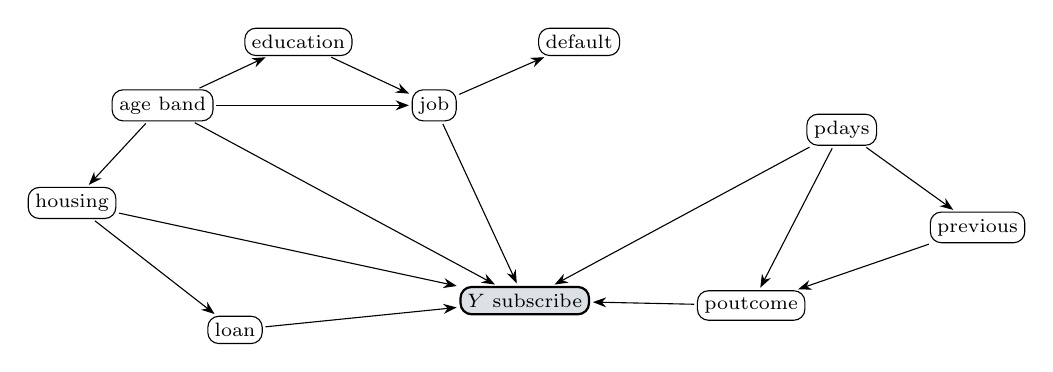
\begin{tikzpicture}[x=1.15cm,y=0.62cm,>=Stealth,
 var/.style={draw,rounded corners,inner sep=2.5pt,font=\scriptsize,fill=white},
 target/.style={draw,rounded corners,inner sep=2.5pt,font=\scriptsize,fill=afgml!15,thick},
 arr/.style={->,shorten >=1pt,shorten <=1pt}]
\node[var] (A) at (0,4) {age band};
\node[var] (E) at (1.5,5.3) {education};
\node[var] (J) at (3,4) {job};
\node[var] (F) at (4.6,5.3) {default};
\node[var] (H) at (-1,2) {housing};
\node[var] (L) at (0.8,-0.6) {loan};
\node[target] (Y) at (4,0) {$Y$ subscribe};
\node[var] (Pd) at (7.5,3.5) {pdays};
\node[var] (O) at (6.5,-0.1) {poutcome};
\node[var] (Pr) at (9,1.5) {previous};
\draw[arr] (A) -- (E);
\draw[arr] (A) -- (J);
\draw[arr] (E) -- (J);
\draw[arr] (J) -- (F);
\draw[arr] (A) -- (H);
\draw[arr] (H) -- (L);
\draw[arr] (Pd) -- (Pr);
\draw[arr] (Pr) -- (O);
\draw[arr] (Pd) -- (O);
\draw[arr] (A) -- (Y);
\draw[arr] (J) -- (Y);
\draw[arr] (H) -- (Y);
\draw[arr] (L) -- (Y);
\draw[arr] (O) -- (Y);
\draw[arr] (Pd) -- (Y);
\end{tikzpicture}
\end{center}
\vspace{-2mm}
\centerline{\small $p(\cdot)=p(A)p(E|A)p(J|A,E)p(F|J)p(H|A)p(L|H)p(P_d)p(P_r|P_d)p(O|P_r,P_d)\,p(Y|A,J,H,L,O,P_d)$}
\begin{itemize}\footnotesize
\item Query and algorithm: $P(Y{=}1\mid e)$, $e$ = observed variables; exact VE (min-fill, min-weight, min-degree) and clique tree (treewidth 6); cost = factor-entry mult + add.
\item Assumptions: associational model, no latent variables; \texttt{unknown} treated as unobserved (A4).
\item Validation: VE vs clique tree vs enumeration, max error $2.2\times10^{-16}$ (tolerance $10^{-6}$), 600 evidence patterns.
\end{itemize}
\end{frame}

\begin{frame}{Fairness criterion and proposed method}
\begin{itemize}
\item Primary fairness criterion: $\Delta_{\mathrm{EOpp}}=\max_g t_g-\min_g t_g$, $t_g=P(D{=}1\mid Y{=}1,G{=}g)$; a missed responder is the harm to the group.
\item Primary utility and allowed loss: average precision (AP), loss $\le0.01$ vs exact (fixed before test).
\item Proposed change: if exact elimination would exceed budget $B$ operations, answer by table lookup; choose $f^\star=\arg\min_f\max_g\mathrm{flip}_g(f)$ s.t.\ validation AP loss $\le0.01$.
\item Protected attribute at prediction time: age band is a model variable (yes); routing is group-unaware; marital status unused.
\item Diagnostics: $\Delta_{\mathrm{DP}}$, $\Delta_{\mathrm{EOdds}}$, fallback-rate gap, decision flips, log loss, Brier.
\end{itemize}
\end{frame}

\begin{frame}{Experimental protocol}
\begin{itemize}
\item Baselines: exact; global fallback; threshold adjustment after budget; fair-adjusted exact; logistic regression; gradient-boosted trees.
\item Matched information and tuning: same variables and splits; thresholds, tables, selection from train/validation only; budget = natural validation op-count quantile (primary 75\%: 11 ops).
\item Selection: capacity 0.2; test protocol frozen in \texttt{docs/protocol.md}.
\item Runs and intervals: 5 seeds (masks, networks, GBT); paired moving-block bootstrap, 1,000 replicates, blocks of 50 date-ordered rows; Holm over 3 comparisons.
\item Mechanism tests: exact agreement; synthetic networks (width $\times$ availability, with control); ablations A1--A4; robustness R1--R6.
\end{itemize}
\end{frame}

\begin{frame}{Main result and uncertainty}
\begin{center}\small\begin{tabularx}{0.95\linewidth}{Xcccc}\toprule
Method & AP $\uparrow$ & $\Delta_{\mathrm{EOpp}}$ $\downarrow$ & Worst-group flip $\downarrow$ & Log loss / Brier $\downarrow$\\\midrule
Exact (reference) & 0.421 & 0.465 & 0 & 0.709 / 0.223\\
Global fallback (baseline) & 0.350 & 0.303 & 0.303 & 0.852 / 0.260\\
Proposed & 0.421 & 0.423 & 0.038 & 0.710 / 0.223\\
Utility-only (A1) & 0.354 & 0.717 & 0.198 & 0.825 / 0.254\\
Threshold adj. & 0.350 & 0.317 & 0.319 & 0.852 / 0.260\\\bottomrule
\end{tabularx}\end{center}
\footnotesize Natural workload, $n=8{,}238$, 11 ops, capacity 0.2; $\Delta_{\mathrm{EOpp}}$ over 7 supported groups.\\[2pt]
\textbf{Paired $\Delta_{\mathrm{EOpp}}$ effect, proposed $-$ comparator (negative favours proposed), 95\% interval:} global $+0.120$ $[0.015,0.226]$, Holm $p=0.036$; utility-only $-0.294$ $[-0.370,-0.210]$, $p=0.006$; threshold adj.\ $+0.106$ $[-0.006,0.251]$, $p=0.080$.\\[2pt]
\textbf{Answer:} hypothesis refuted. Proposed keeps exact decisions (98.3\% agreement, AP loss 0), but global and threshold baselines reach lower $\Delta_{\mathrm{EOpp}}$ only by levelling down (AP $-0.071$).
\end{frame}

\begin{frame}{Ablation, robustness and failure case}
\begin{columns}[T]
\begin{column}{0.58\textwidth}\footnotesize
\begin{itemize}
\item Ablation A1 (no fairness-aware selection): worst flip $0.038\to0.198$, $\Delta_{\mathrm{EOpp}}$ $0.294$ worse. A3 (no simplification): fallbacks $20.1\%\to26.2\%$, AP $0.421\to0.356$. A4 (258 ops): no fallbacks, exact behaviour.
\item Robustness: capacity 0.1/0.3 and elimination orders keep the pattern; dense / sparse networks raise proposed worst flip to $0.206$ / $0.133$.
\item Failure case (synthetic dependent masks, exploratory): proposed picks the age-based fallback in 3 of 5 seeds, AP loss $0.046$, $\Delta_{\mathrm{EOpp}}$ $+0.493$ $[0.397,0.569]$ vs exact; group-unaware variant loses $0.003$ AP.
\item Interpretation: bootstrap intervals are sampling uncertainty of fixed models; seed and scenario variation is separate; the simulation is not customer fact.
\end{itemize}
\end{column}
\begin{column}{0.4\textwidth}
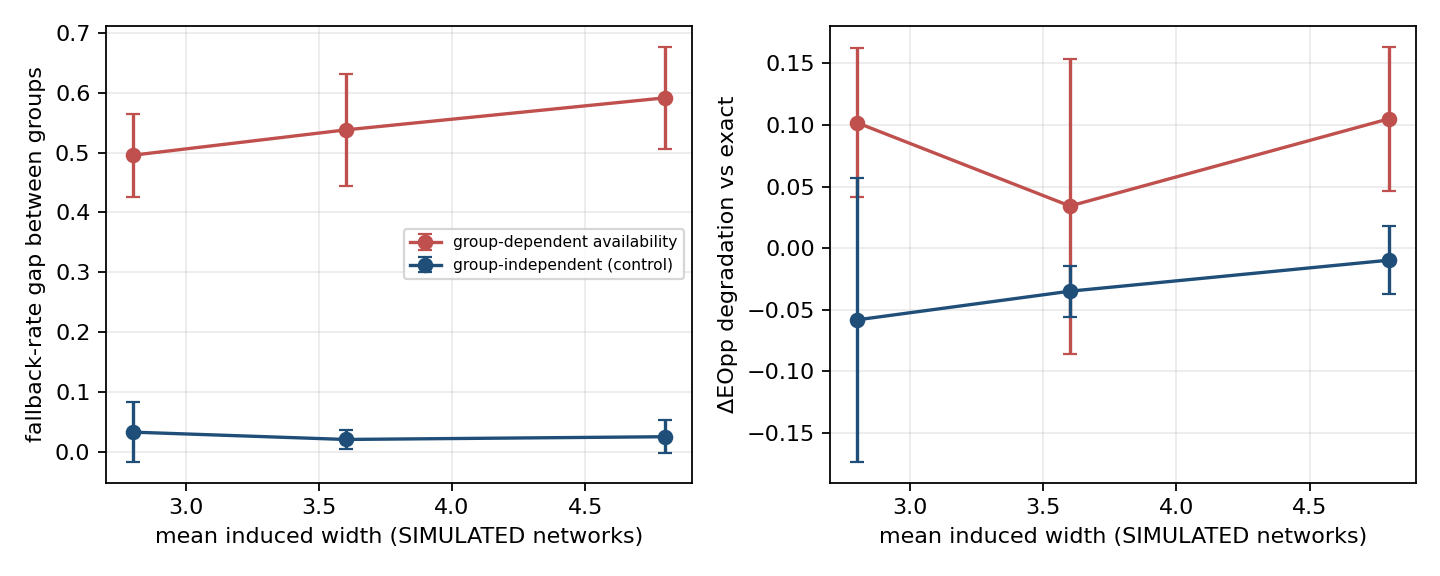
\includegraphics[width=\linewidth]{results/figures/fig_synthetic_mechanism.png}\\
{\scriptsize SIMULATED networks: fallback-rate gap $0.542$ (group-dependent) vs $0.026$ (control).}
\end{column}
\end{columns}
\end{frame}

\begin{frame}{Conclusion and reproducibility}
\begin{itemize}
\item Conclusion: fairness-aware selection preserves exact decisions at a tight budget, but does not give the smallest $\Delta_{\mathrm{EOpp}}$; the confirmatory hypothesis is refuted.
\item Limits and ethics: base rate drifts $4.8\%\to30.8\%$ (test selection 38.3\% vs 20\%); no customer ids; contacted-only sample; 5 exploratory groups; simulations labelled.
\item Reproduce: \texttt{scripts/run\_experiments.py --mode real}, \texttt{evaluate.py --out results}, \texttt{make\_results.py --out results --mode real}; \texttt{configs/main.yaml}; commit \texttt{e2350bcd6d58}.
\item Shreeya Kamath: implementation (inference, baselines, experiments, notebook) and slide alignment.
\item Misha: debugging, report writing and slides. Each cross-checked the other's work (\texttt{docs/contributions.md}).
\end{itemize}
\end{frame}
\appendix
\begin{frame}{Backup: mandatory evidence and references}
\footnotesize
\begin{tabularx}{\linewidth}{llXl}\toprule
ID & Requirement & Artifact (\texttt{results/metrics/}) & Status\\\midrule
C-GM & VE = clique tree = enumeration & \texttt{exp1\_exact\_agreement.json}, \texttt{cgm.json} & complete\\
C-STAT & Paired block bootstrap, Holm & \texttt{bootstrap.csv} & complete\\
Exp 2 & Cost, peak factor, memory & \texttt{exp2\_complexity.csv} & complete\\
Exp 3--4 & Budgets, matched utility, baselines & \texttt{main\_results.csv}, \texttt{group\_table.csv}, \texttt{predictive\_baselines.csv} & complete\\
Exp 5 & Synthetic networks with control & \texttt{exp5\_aggregate.csv}, \texttt{exp5b\_factorial.csv} & complete\\
A1--A4, R1--R6 & Ablations, robustness & \texttt{main\_results.csv} (tags) & complete\\
Latency & Wall-clock, separate & \texttt{latency.csv} & complete\\\bottomrule
\end{tabularx}\\[4pt]
Das, Romanelli, Fioretto, ICML 2024 (arXiv:2402.03629); Hardt, Price, Srebro, NeurIPS 2016 (arXiv:1610.02413); Moro, Rita, Cortez, UCI dataset 222; Koller \& Friedman, \emph{Probabilistic Graphical Models}, MIT Press 2009. Full table: \texttt{docs/related\_work.md}; manifest: \texttt{results/manifest.csv}.
\end{frame}
\begin{frame}{Backup: inference and statistical validation}
\footnotesize
\begin{itemize}
\item Factor scopes: every CPD normalises over its child (checked). Maximal cliques (min-fill): $\{A,E,J\}$ 288 entries; $\{A,H,J,L,P_d,Y\}$ 3,888; $\{F,J\}$ 36; $\{P_d,O,P_r\}$ 12; treewidth 6.
\item Exact agreement: max $|\mathrm{VE}-\mathrm{CT}|=2.2\times10^{-16}$, vs enumeration $1.1\times10^{-16}$ (tolerance $10^{-6}$); 20 random 8-node networks $\times$ 10 queries $\times$ 3 heuristics also pass.
\item Cost (natural evidence): VE mean 24.7 ops, peak factor 96; clique-tree calibration 44,790 ops per evidence (+29,337 preprocessing); wall-clock 0.225 vs 1.09 ms per query.
\item Test denominators (positives / $n$): 30--59 married 932/3,152; $<30$ single 502/1,525; 30--59 single 451/1,631; $\ge60$ married 309/659; 30--59 divorced 176/650; $\ge60$ divorced 70/160; $<30$ married 79/384. Exploratory: $<30$ divorced 6/34; $\ge60$ single 8/25; 30--59 unknown 5/14; two unknown cells 1/2.
\item Bootstrap: moving blocks of 50, 1,000 replicates, 95\% percentile, statistic $\Delta_{\mathrm{EOpp}}$ over the 7 supported groups; Holm family = 3 comparisons (natural workload). All-group sensitivity intervals are wide (e.g.\ vs global $-0.167$ $[-0.385,0.554]$).
\end{itemize}
\end{frame}
\begin{frame}{Backup: demonstration and individual defence}
\small
\begin{itemize}
\item Command: \texttt{python scripts/evaluate.py --out results \&\& python scripts/make\_results.py --out results --mode real} regenerates the bootstrap table and main table from saved runs (about 40 s); the full run took 1,307 s (Python 3.13, Linux).
\item Saved trace (most expensive natural query; observed: age 30--59, default no, housing no, loan no, poutcome failure): min-fill eliminates previous\_bin (6 ops), education (180), job (140), pdays\_bin (8); total 339 ops; $P(Y{=}1\mid e)=0.1683$.
\item Same posterior by min-degree order (339 ops) and by clique-tree calibration (41,325 ops); order changes cost, never the posterior.
\item Be ready to: trace one operation count; justify $\Delta_{\mathrm{EOpp}}$ and why levelling down matters; critique the claim given base-rate drift and tiny groups.
\end{itemize}
\end{frame}
\end{document}
